\documentclass[12pt]{article}
\setlength{\oddsidemargin}{0in}
\setlength{\evensidemargin}{0in}
\setlength{\textwidth}{6.5in}
\setlength{\parindent}{0in}
% \setlength{\parskip}{\baselineskip}
\usepackage{graphicx}
\usepackage{multirow}
\usepackage{multicol}
\usepackage{listings}
\usepackage{color}
\rmfamily
\definecolor{dkgreen}{rgb}{0,0.6,0}
\definecolor{gray}{rgb}{0.5,0.5,0.5}
\definecolor{mauve}{rgb}{0.58,0,0.82}

\lstset{frame=tb,
  language=R,
  aboveskip=3mm,
  belowskip=3mm,
  showstringspaces=false,
  columns=flexible,
  basicstyle={\small\ttfamily},
  numbers=none,
  numberstyle=\tiny\color{gray},
  keywordstyle=\color{blue},
  commentstyle=\color{dkgreen},
  stringstyle=\color{mauve},
  breaklines=true,
  breakatwhitespace=true,
  tabsize=3
}

\usepackage{amsmath,amssymb,amsrefs}
\usepackage[top=24mm, bottom=18mm, left=15mm, right=13mm]{geometry}
\usepackage{url}

\begin{document}
\begin{center}
{\bf Homework 3}\\
{\bf MATH 191 Topics in Data Science}\\
\end{center}

1a. 
\begin{align} \nonumber
\mathbb{E}[\mu_n] &= \mathbb{E}[\frac{1}{n}\sum_{k=1}^nx_k] \\ \nonumber
&= \mathbb{E}[\frac{1}{n}]\mathbb{E}[x_1 + x_2 + \dots + x_n] \\ \nonumber
&= \frac{1}{n}(\mathbb{E}[x_1] + \mathbb{E}[x_2] + \dots + \mathbb{E}[x_n]) \\ \nonumber
\end{align}
\begin{center}
Since $x_1, x_2, \dots, x_n$ are independent identically distributed, they have have the same expected value $\mu$, thus:
\end{center}
\begin{align} \nonumber
\mathbb{E}[\mu_n] &= \frac{1}{n}n\mu \\ \nonumber
\mathbb{E}[\mu_n] &= \mu
\end{align}
1b. 
\begin{align} \nonumber
\mathbb{E}[H] &= \mathbb{E}[\frac{1}{n-1} \sum_{k=1}^n (x_k - \mu_n) (x_k - \mu_n)^T] \\ \nonumber
&= \frac{1}{n-1} \sum_{k=1}^n \mathbb{E}[(x_k - \mu_n) (x_k - \mu_n)^T] \\ \nonumber
&= \frac{1}{n-1} \sum_{k=1}^n\sum_{j=1}^{n-1} (\mathbb{E}\mu_n^2 - \mu^2) \\ \nonumber
&= \frac{1}{n-1} n(n-1)Var(\mu_n) \\ \nonumber
&= \frac{1}{n-1} (n-1)C \\ \nonumber
&= C
\end{align}
\newpage
2. 
a. The code for run\_PCA is as follows:
\begin{lstlisting}
run_PCA = function(X_train) {

# Training X matrix: X_ train of size n by p

myPCA = prcomp(X_train, center = TRUE, scale. = TRUE, retx = TRUE);
print(summary(myPCA));
t5load = myPCA$x[,1:5];
return(t5load);
}

# This is the updated main_linear_regression() function
PCARet = run_PCA(RET);
X_train = PCARet[1:(nrDays-1),];
X_test = PCARet;
STATS = NULL;
#CM = NULL;

for (i in 1:nrTickers) {
	print('#############################################');
	print( paste('Stock = ',tickers[i] ) );
	y_train = RET[ 2 : nrDays , tickers[i], drop=FALSE];  # "drop=FALSE" ensurs it remains a 2-D array..

	y_hat = compute_linear_regression(X_train, y_train, X_test);
	# compute the various performance statistics:
	
	daily_pnl = matrix(, nrow = nrDays - 1, ncol = 1);
	for (j in 1:(nrDays - 1)) {
		if (y_hat[j] < 0) {
			daily_pnl[j] = -RET[j+1,i]
		}
		else {
			daily_pnl[j] = RET[j+1,i];
		}
	}
	cum_pnl = cumsum(daily_pnl);
	#CM = cbind(CM,cum_pnl);
	mean_pnl = mean(daily_pnl, na.rm=TRUE);
	yearly_pnl = mean(daily_pnl, na.rm=TRUE) * 252;
	total_pnl = sum(daily_pnl, na.rm = TRUE);
	sharpe = compute_Sharpe_Ratio(daily_pnl);
	
	stats_this_stock = c(sharpe, mean_pnl, yearly_pnl, total_pnl)
	STATS = rbind(STATS,stats_this_stock);

	readline('Press key to continue...');
}
\end{lstlisting}
\hfill \break
The top five components captured variance is about 90\%:
\begin{lstlisting}
Importance of components:
                         PC1    PC2    PC3     PC4     PC5
Proportion of Variance 0.491 0.1736 0.1002 0.07558 0.05788 = 0.89826
\end{lstlisting}

b. Using PCA and in-sample linear regression:
\begin{lstlisting}
         sharpe     mean_pnl yearly_pnl total_pnl
SPY   0.5266759 0.0003336390 0.08407702 0.4210524
^VIX  0.8622320 0.0040718819 1.02611424 5.1387149
^TNX  0.3908225 0.0005656769 0.14255057 0.7138842
OIL   0.9089427 0.0010815811 0.27255843 1.3649553
GOLD  1.0403505 0.0015117883 0.38097065 1.9078768
^N225 5.8604248 0.0047542839 1.19807954 5.9999063
^FTSE 3.1129761 0.0019194213 0.48369416 2.4223096
GLD   0.6345453 0.0004399835 0.11087584 0.5552592
SPXS  1.2072723 0.0023141396 0.58316318 2.9204442
SPXL  0.4458274 0.0008583874 0.21631362 1.0832849
=================================================
AVG   1.4990069 0.0017850783 0.44983972 2.2527688
\end{lstlisting}
\hfill \break
c. Using PCA and out-sample linear regression:
\begin{lstlisting}
# This is the updated main_linear_regression() function
	for (i in 1:nrTickers) {

		daily_pnl = matrix(, nrow = nrDays - 101, ncol = 1);

		for (j in 101: (nrDays - 1)) {
			y_train = RET[ (j - 99) : j , tickers[i], drop=FALSE];
			X_train = RET[ (j - 100) : (j - 1) ,]
			X_test = RET[j,];
			Q = rbind(X_train, X_test);
			Qt = run_PCA(Q);
			Xt_train = Qt[1:100,];
			Xt_test = Qt[101, ,drop = FALSE];
			y_hat = compute_linear_regression(Xt_train, y_train, Xt_test);
			if(y_hat < 0) {
				daily_pnl[j - 100] = -RET[j + 1, i];
			}
			else {
				daily_pnl[j - 100] = RET[j + 1, i];
			}
		}
		mean_pnl = mean(daily_pnl, na.rm=TRUE);
		yearly_pnl = mean(daily_pnl, na.rm=TRUE) * 252;
		total_pnl = sum(daily_pnl, na.rm = TRUE);
		sharpe = compute_Sharpe_Ratio(daily_pnl);
		stats_this_stock = c(sharpe, mean_pnl, yearly_pnl, total_pnl)
		STATS = rbind(STATS,stats_this_stock);
	}
\end{lstlisting}
\begin{lstlisting}
           sharpe      mean_pnl  yearly_pnl  total_pnl
SPY   -0.42483859 -0.0002630994 -0.06630105 -0.3057215
^VIX  -0.27237255 -0.0012693194 -0.31986848 -1.4749491
^TNX   0.23200048  0.0003427176  0.08636484  0.3982379
OIL   -0.20493539 -0.0002444066 -0.06159045 -0.2840004
GOLD  -0.35436615 -0.0005135521 -0.12941512 -0.5967475
^N225  5.45665707  0.0044504105  1.12150345  5.1713770
^FTSE  1.67787593  0.0010291882  0.25935542  1.1959167
GLD   -0.24228651 -0.0001684264 -0.04244346 -0.1957115
SPXS  -0.09852636 -0.0001848992 -0.04659460 -0.2148529
SPXL  -0.43634300 -0.0008222165 -0.20719855 -0.9554155
======================================================
AVG    0.53328649  0.0002356397  0.05938120  0.2738133
\end{lstlisting}
\hfill \break
We see that the out-sample analysis using the sliding window approach gives a much lower average for our profit. Many of the instrument's Sharpe Ratios fall below 0. However, this result should fit more accurately than our in-sample analysis with its over-fit values. We would also still make a net profit with the forecast model.
\\ \\
d. Using knn-regression:
\begin{lstlisting}
           sharpe      mean_pnl  yearly_pnl   total_pnl
SPY    0.12984995  8.044124e-05  0.02027119  0.09347272
^VIX   0.16864502  7.859963e-04  0.19807108  0.91332774
^TNX   0.12552468  1.854426e-04  0.04673154  0.21548430
OIL   -0.08910839 -1.062781e-04 -0.02678209 -0.12349517
GOLD  -0.21211124 -3.074436e-04 -0.07747578 -0.35724943
^N225  4.75759522  3.930419e-03  0.99046558  4.56714685
^FTSE  1.00264345  6.172068e-04  0.15553612  0.71719432
GLD   -0.81183224 -5.636769e-04 -0.14204657 -0.65499253
SPXS  -0.02379274 -4.465138e-05 -0.01125215 -0.05188491
SPXL  -0.05639919 -1.063145e-04 -0.02679125 -0.12353742
=======================================================
AVG    0.49910145  4.471142e-04  0.11267277  0.51954665
\end{lstlisting}
\hfill \break
Using k nearest neighbors regression, we have a much tighter result with lower averages across the board except for total pnl, which indicates that this forecast would have resulted in a better profit than using linear regression. 
\newpage
e. \\
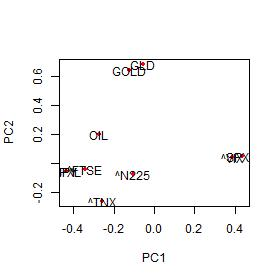
\includegraphics{plots1.jpeg}
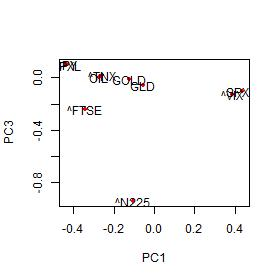
\includegraphics{plots2.jpeg} \\
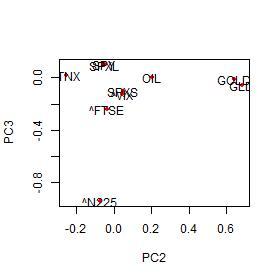
\includegraphics{plots3.jpeg} \\
\newpage
3.\\
a. It can be seen that most of the eigenvalues are close to 0, with a few sporadically appearing up to 0.03. Eigenvalshrunk contains all eigenvalues less than 0.002, which contains 466 of the of 472 eigenvalues. 
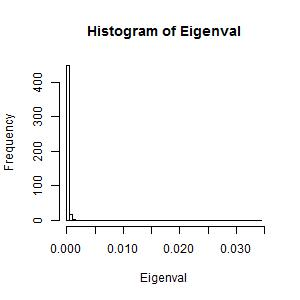
\includegraphics[scale = .9]{eighist1.jpeg}
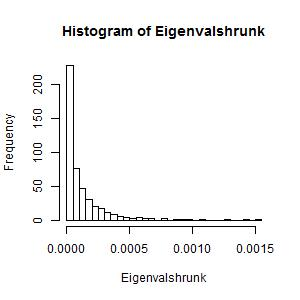
\includegraphics[scale = .9]{eighist2.jpeg} \\
\\b. randEig is the average eigenvalue of the 50 iterations of randomizing RETS, giving the histogram: \\
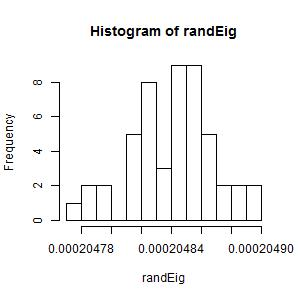
\includegraphics{eighist3.jpeg} \\
\newpage
c. Using $max(Eigenval)$ and $max(randEig)$, we get:
\begin{lstlisting}
> max(Eigenval)
[1] 0.03429729
> max(randEig)
[1] 0.0002048967
\end{lstlisting}
\hfill \break
d. We can see that the distributions are quite similar, with randEig being more evenly distributed in its 0.0002 range and Eigenval being a little more sparsely distributed but in the similar region.
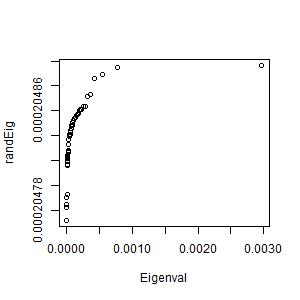
\includegraphics[scale = .8]{qqplot.jpeg}
\centering
\\
e. The averages found in (b) do not make up the largest 20 in our actual eigenvalues. Due to a varying set of both very small and extremely large eigenvalues, are average in this case does not align with our actual data. \\
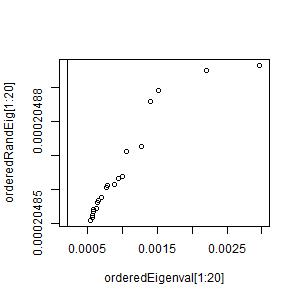
\includegraphics[scale = .8]{eigscatter.jpeg}
\centering
\end{document}